\documentclass[12pt,a4paper]{article}
\usepackage[utf8]{inputenc}
\usepackage[english]{babel}
\usepackage[]{fullpage}
\usepackage{graphicx}


\title {Abacus \\ Interpreter for mathematical expressions in SML}
\author{
  Vågbratt, Tommy
  \and
  Loberg, Micael
	\and
  Jin, Wenting}
\date{\today}


\begin{document}

\maketitle
\tableofcontents
\newpage


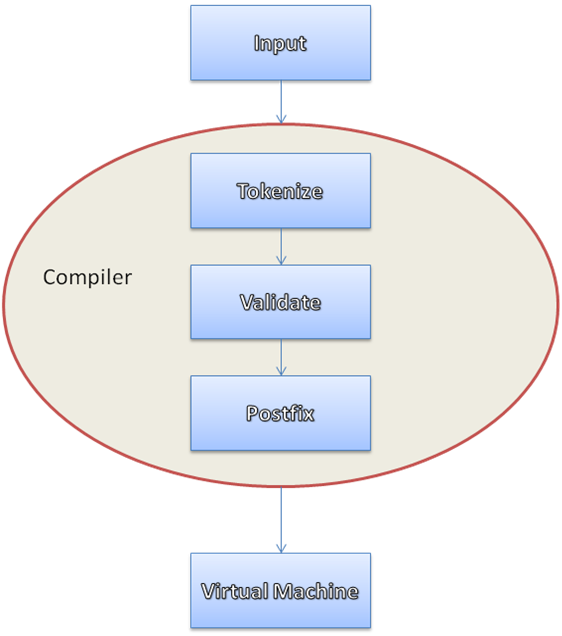
\includegraphics[width=\textwidth]{Structure}

\section{Introduction}
\textnormal{A tool that takes mathematical expressions in text form may sound nothing special, but one may have encountered difficulties to find the right symbol on a typing-in calculator to express trigonometric related functions such as "sin", "arctan" etc. However, this program (Abacus) performs as an interpreter and functions just as a "normal" calculator, but can evaluate a whole mathematical expression that is just based on text! No more time wasting looking up symbols, with ability to declare variables, to do more advanced calculation. Interesting? Well, it's just a "calculator".}

\section{"Calculator" in SML}
\subsection{Design and Structure}
\textnormal{There are three major parts of the system: Input, Compiler and Evaluation which are combined into a REPL\footnote{Read-Evaluate-Print Loop, more about REPL, please refer to http://en.wikipedia.org/wiki/REPL}. All these parts are strictly sequential between each other. All steps inside a part are to build preparation work for next part, and all three parts form a successive execution. Executions can be achieved as many times as user need.}
\subsubsection{Structure Overview}
\begin{description}
  \item [Input] \hfill \\Handles input text, takes the input and passes it to the compiler.
  \item [Compiler] \hfill
  \begin{itemize}
    \item Tokenize: Takes an expression represented as a string and split it into Tokens.
    \item Validate: Performs grammatical validation on tokens, but careless of priority of the functions/operators \change
    \item Translate: Convert an expression represented by Tokens from infix notation to postfix notation with priority considered \change
  \end{itemize}    
  \item [Evaluation] \hfill \\ Compiled expression gets evaluated. A stack based "virtual Machine" evaluates the expression using the following rules:
  \begin {itemize}
    \item Numbers are pushed onto the stack.
    \item Variables are looked up and get pushed onto the stack.
    \item Functions and operators takes item(s) off from the stack and push the evaluated result back onto the stack
  \end {itemize}
\end{description}


\iffalse
En mer detaljerad beskrivning (design)
- Vilka delar består systemet av? Hur samverkar de för att lösa problemet?

- Vilka datastrukturer används? Beskriv abstrakta datatyper (gränssnitt/interface)
\fi

\subsection{Algorithms and Alternatives}
\textnormal{ Data-types used in this program: Stack, Token, Environment.}
\begin{description}
  \item [Stack] is a data-structure that only has three operations, pushing (adding) data to the top and the stack, and popping (removing) 
  data from the top of the stack, and reading the top element of the stack without modifying the stack.

  \item[Token] is the data-structure used in the program to represent numbers, functions, variables, parentheses and operators.

  \item[Enviroment] is a list of variables and their values.
\end{description}

\subsubsection{Tokenize}
\textnormal{An expression can consist of number, assignment, identifiers of variable, operator and function, open and close parenthesis and whitespace. Tokenize takes expression represented as a string and splits them into token characterized as Number, Variable, Assignment, Function, Operator, Open and Close parenthesis}
\begin{itemize}
\item Number:
\begin {enumerate}
\item \emph{Start}: take in digit 0-9.
\item if 0 encountered, either is a 0, \emph{or} followed by a decimal point with 0-9 combinations
\item if 1-9 encountered, either \emph{1)}:followed by 0-9 combinations \emph{or} \emph{2)}: 0-9 combinations followed by a dot(.) with 0-9 combinations \emph{or} \emph{3)}: followed by decimal point with 0-9 combinations
\end{enumerate}
\item Identifier:
\begin {enumerate}
\item \emph{Start}: take in alphabet a-z, A-Z until first digit 0-9 encountered
\item check if exist in function or operator list
\begin {itemize}
\item if exist recognized as an operator or a function, terminate and back to \emph{Start}
\item if not exist in list, take in the digit encountered and keep on reading a-z, A-Z, 0-9
\end{itemize}
\end{enumerate}
\item Symbolic Operator: take in symbolic operator (such as. *,/,+,-, etc)
\item Parentheses
\begin{itemize}
\item take in left parenthesis (, terminate and back to \emph{Start}
\item take in right parenthesis ), terminate and back to \emph{Start}
\end{itemize}
\item Whitespace: whitespace “ “ encountered, terminate and back to \emph{Start}
  
\end{itemize}

\subsubsection{Validate}
textnormal{
\begin {enumerate}
Validate is achieved with recursive descent parser. \newline 
Validate is implemented using a recursive descent parser algorithm.
It is made from a number of mutually recursive states, the states being:

\newline A has two constructs, either Variable = A, or E}
\newline E is an expression and has two constructs, N op E, and N
\newline N also has two constructs, either its T, or –T
\newline T the  
\begin {itemize}
  \item A \Rightarrow Var = A | E
  \item E \Rightarrow N op E | N
  \item N \Rightarrow T | -T
  \item T \Rightarrow Num | Var | fun N | (E)
\end{itemize}
\end{enumerate}

\subsubsection{Translate}
\textnormal{The method for converting an expression in infix notation to postfix notation makes use of two lists, the first one holding the input and the second one holding the output, and a stack that holds the operators, functions and parentheses. 
This algorithm is called the \emph{Shunting-yard algorithm} and was invented by \emph{Edsger Wybe Dijkstra}\cite{dijkstra}.

}
}
\subsubsection{Evaluate}
\textnormal{Evaluate is implemented with an algorithm that makes use of an Enviroment, a stack and a list containing the input.
It takes a list of Tokens as input, a stack and an enviroment that holds all the variables.
After the evaluation is done the result will be added to a Variable called "ans" that is inserted into the Enviroment
}


\subsubsection{Alternative algorithms}
\textnormal{There are other ways of evaluating mathematical expressions. Instead of first converting the expression from infix notation to postfix 
notation using the \emph{shunting-yard algorithm} and then evaluating it, an abstract syntax tree could be built while reading the input.
That could be achieved with an algorithm similar to the one used
in this program to validate the expression. That is, using an \emph{top down recursive descent algoithm}\cite{rda}
If an abstract syntax tree was used the expression could then be evaluated by simple traversing the tree and evaluate the operators
and functions as they are encountered.

The main reason for chosing to first convert it from postfix to infix notation before evaluating the expression is that it would be easier for
us to implement it compaired to building an abstract syntax tree.
Another reason for our choice of algorithms is that the method of converting an expression from infix notation to postfix notation and then 
evaluating it was briefly mentioned during one of the lectures which sparked an interest for this project.

In the end both methods would give the same result, and for our purpuse our method is fast enought.}
\iffalse
Smarta lösningar (algoritmer)
- Beskriv viktiga funktioner Designval
- Finns alternativa sätt att lösa problemet? Varför valde du det här sättet?
- Konsekvenser av dina val

\fi

\subsection{Implementation}
\textnormal{Logotype is presented and there is a user manual built into the program, by typing “help”, user can get user guide on how to use the program. \newline \newline Test cases are included for every source code file. \newline \newline It is easy to add more support for functions and operators because priority is not part of the validation but is handled in the translation part.}

\subsubsection{Tokenize implemitation}
\textnormal{
 
}
\subsubsection{Validate implemetation}
\textnormal{
Validate is implemented using a recursive descent parser algorithm.
It is made from a number of mutually recursive states
}
\subsubsection{Translate implemetation}
\textnormal{
The algorithm is implemented like this in pseudo-code:
}

\begin{itemize}
  \item While input is not empty, read a Token
\begin{itemize}
    \item If Token is a number or a variable, add it to the output list
    \item If Token is a left parenthesis, add it to the operator stack
    \item If Token is a function or an operator, check the priority of the top element of the operator stack.
    \begin{itemize}
      \item if the operator/function on the top of the stack has higher or equal priority to Token, 
      push it to the output list, repeat until Token has lower priority than the top element of the stack.
      \item if priority of Token is higher, put it on the output list
    \end{itemize}
    \item If Token is a right parenthesis, pop elements off the stack to the output list until a left 
    parenthesis is found, then discard both the left and right parenthesis.
    \item If the input list is empty:
    \begin{itemize}
      \item While the stack is not empty:
      \begin{itemize}
        \item Pop elements off the stack to the output list.
      \end{itemize}
    \end{itemize}
    \item if both the input list and the stack are empty:
    \begin{itemize}
      Reverse the output list.
    \end{itemize}
\end{itemize}
\textnormal{
  The expression has now been converted from infix notation to postfix notation and is now ready to be evaluated.
}
\subsubsection{Evaluate implemetation}
\textnormal{
  The algorithm is implemented like this in pseudo-code:}
\begin{itemize}
  \item While input is not empty, read a Token
  \begin{itemize}
    \item If Token is a number then push the value of the number to the stack.
    \item If Token is a variable 
    \begin{itemize} 
      \item Get the value for the variable from the Enviroment and push it to the stack.
      \item If the variable can't be found in the Enviroment it is undefiened, raise an exception.
    \end{itemize}
    \item if Token is a function or operator, pop off as many arguments as the function needs from the stack, evaluate the function 
    and push the result back to the stack.
  \end{itemize}
  \item If input is the empty list, then everything on the stack has been evaluated and only has one element,
  this element is the result.
\end{itemize}
After the expression has been evaluated, the result is put in to the environment as the variable “ans”.
}
\iffalse

- Intressanta detaljer
- Fungerar programmet? Hur vet du det?
- Finns det saker som inte fungerar, fall som inte hanteras?
- Ãr programmet effektivt?
\fi

\subsection{General Analysis}
\textnormal{Abacus is a tool with feature of being handy and flexible, though user might find it clueless when error message happens. When expressions become long and more advanced, it can be more time-consuming to get result.}
\iffalse
Analys/diskussion
- Vilka Ãr systemets styrkor/svagheter? -> Sustainability
- Blev det bra? Skulle du ha gjort något annorlunda om du skulle börja om? -> Sustainability
- Tänkbara vidareutvecklingar -> Furture Development
\fi

\subsubsection{Furture Development}
\textnormal{
Even though the project started out as an idea to make a simple calculator it has become quite powerful.
The user is able to to use most functions available on expensive calculators and store variables for later use
with a user friendly interface.
The program can very easily be expanded upon since the way functions and operators are stored is very flexible.
Allowing the user to define functions could be implemented without much effort, unfourtunitly this is a feature that had
to be skipped due to time constraints, but it would be implemented in a similar fashion to variable assignment.
}


\subsubsection{Sustainability}
\textnormal{
One major flaw in the program is that error messages aren't always very descriptive.
The reason for this is that handling exceptions in Standard ML can be a bit tricky.
Another side effect of it being hard to handle exceptions is that in order to keep the main loop running when 
exceptions are raised a new instance of the main function are run on top of it. 
This could in theory make the program crash as the available memory would be depleted, though this would take a very long time.  
}


\section{Conclusion}
\textnormal{
We picked this project knowing that we would be in for a challange.
Before we could start writing the code we had to read about different ways
of solving the problems we expected to encounter.
Writing the parser that is used in the Validate part was especially problamatic but by
reading more about top down recursive algorithms we managed to solve it.

In the end we are very satisfied with the result, it is a very functional program that has almost all of the features
we had planned for.
}
\iffalse
- Avslutning: Sammanfattning, diskussion, slutsatser
\fi

\section{Simple Guide for Simple Calculator}
\textnormal{ 
Upon starting the application the user will be presented with a command line interface.
The user simply types in the expression that is to be evaluated.

Typing "help" in the prompt will show a brief overview of the available functions, operators and default variables (such as Pi, e).
Typing "logo" will display the logo for Abacus.
Typing "credits" will display information about the creators of the program.
}
\subsection{Examples}
\textnormal{
  To evaluate the expression $3+(3 \cdot 4)$ simply input the expression in the prompt.
  To use the sin function, simply type $sin~ expression$ where $expression$ can be any expression.
  To assign a variable to the value of the same expression, type
  $x = 3+(3 \cdot 4)$, where x can be any identifier.

  To get the value of the previous evaluated expression typ "ans".
}
\iffalse
- Användarhandledning med exempel (use cases)
\fi



\begin{thebibliography}{breitestes Label}
\bibitem{dijkstra}
  % info...
  MR 34/61
  Algol 60 translation : An algol 60 translator for the x1 and making a translator for algol 60
  1961
  \emph{}
	
\bibitem{rda}
  Alfred Aho, Monica Lam, Ravi Sethi, Jeffry Ullman \\
  Compilers: Principles, techniques and tools, second edition. Chapter 5, page 338 \\ 
  Pearson internation edition 2006 \\
  ISBN: 978-0-321-49169-5
	
\end{thebibliography}



\end{document}
